\section{The Particle Flow Algorithm}


The information available from all CMS subdetectors is employed in the particle-flow (PF) algorithm \cite{CMS:2009nxa,CMS:2010byl} to identify and reconstruct individual particles in the event, namely muons, electrons, photons, and charged and neutral hadrons. These particles are used to reconstruct jets, \hadtau candidates, and the vector imbalance in transverse momentum in the event, referred to as \ptvecmiss, as well as to quantify the isolation of leptons. 

\subsection{Electrons reconstruction}
Electrons are reconstructed by matching tracks in the inner detector with energy depositions in the ECAL \cite{CMS:2009nxa,Baffioni2007}. The tracks of electron candidates are reconstructed using a Gaussian sum filter \cite{Adam:2005bya} algorithm, which accounts for the emission of bremsstrahlung photons along the electron trajectory. Energy loss in bremsstrahlung is reconstructed by searching for energy depositions in the ECAL located in directions tangential to the electron track. A multivariate approach based on boosted decision trees (BDT) \cite{Hocker:2007ht} is employed for electron identification \cite{1748-0221-10-06-P06005}.

\subsection{Muons reconstruction}

 The identification of muons is based on linking track segments reconstructed in the silicon tracking detector and in the muon system \cite{Chatrchyan:2012xi}. The matching between track segments is done outside-in, starting from a track in the muon system, and inside-out, starting from a track reconstructed in the inner detector. In case a link can be established, the track parameters are refitted using the combined hits in the inner and outer detectors, with the resulting track referred to as a global muon track. Quality criteria are applied on the multiplicity of hits, on the number of matched segments, and on the fit quality of the global muon track, quantified through a \ensuremath{\chisquare}.

\subsection {The Jet reconstruction}

Jets within the range \ensuremath{|\eta| < 4.7} are reconstructed using the anti-\ensuremath{k_{T}} algorithm \cite{antikt} with a distance parameter of 0.5. As mentioned previously,the particles reconstructed by the PF algorithm are used as input to the jet reconstruction. Reconstructed jets are required not to overlap with identified electrons, muons, or τh within \ensuremath{\Delta R < 0.5}, and to pass two levels of jet identification criteria: (i) misidentified jets, mainly arising from calorimeter noise, are rejected by requiring reconstructed jets to pass a set of loose jet identification criteria \cite{CMS:2010xta} and (ii) jets originating from pileup interactions are rejected through an MVA-based jet identification discriminant, relying on information about the vertex and energy distribution within the jet \cite{CMS:2013wea}. The energy of reconstructed jets is calibrated as a function of jet \pt and \ensuremath{\eta} \cite{1748-0221-6-11-P11002}. The contribution of pileup to the energy of jets originating from the hard scattering is compensated by determining a median transverse momentum density (\ensuremath{\rho}) for each event, and subtracting the product of ρ times the area of the jet, computed in the \ensuremath{\eta-\Phi} plane,from there constructed jet pT \cite{Cacciari:2008gn, Cacciari:2007fd}. Jets originating from the hadronization of b quarks are identified through the combined secondary vertex (CSV) algorithm \cite{Chatrchyan:2012jua}, which exploits observables related to the long lifetime of b hadrons and the higher particle multiplicity and mass of b jets compared to light-quark and gluon jets.

\begin{figure}
	\centering
	\begin{subfigure}{1\textwidth}
		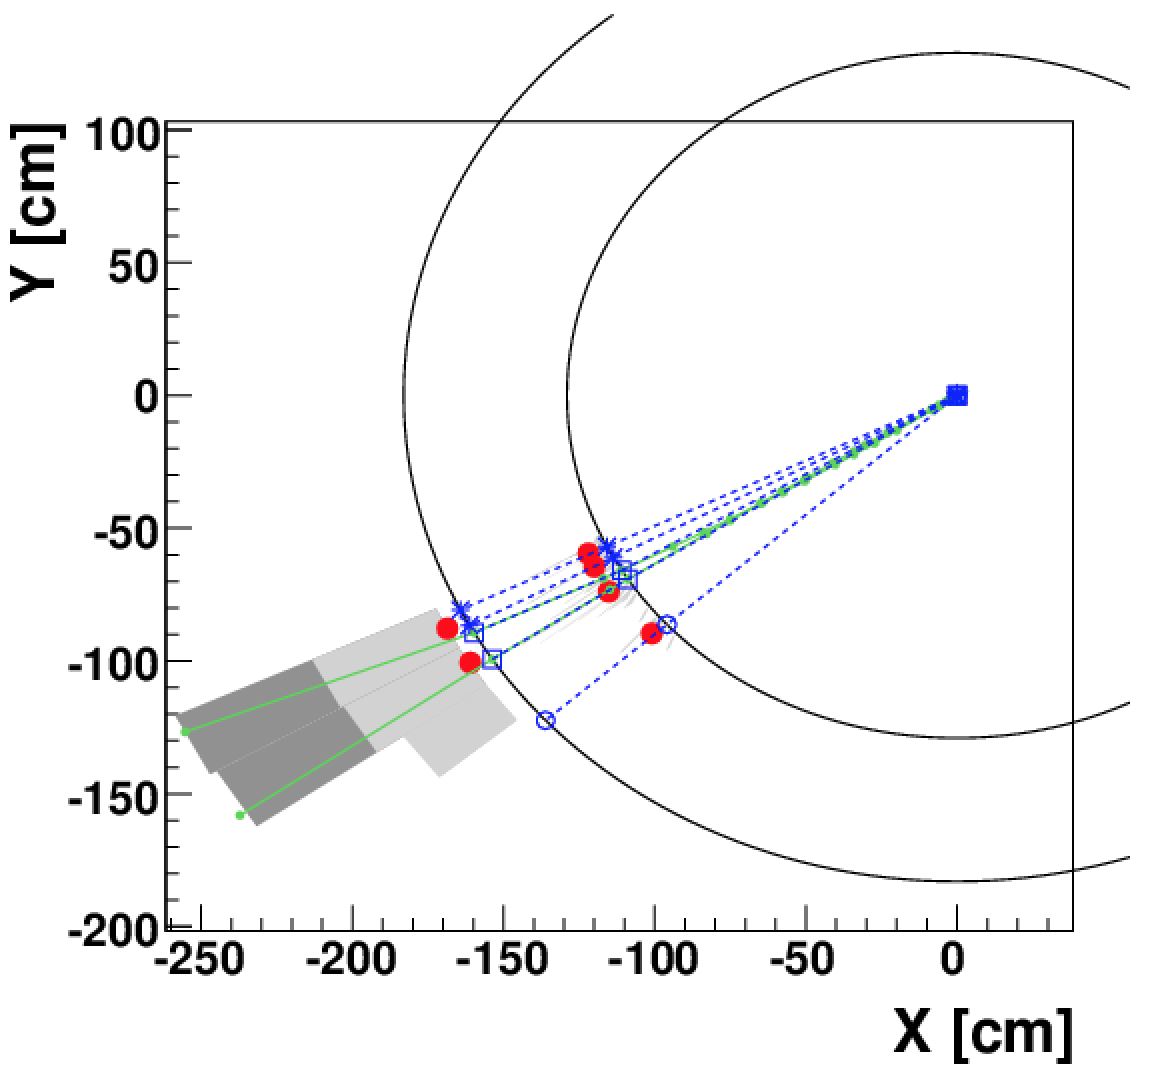
\includegraphics[width=.8\linewidth]{analysis/pics/PF_a.png}
		\caption{The $(x, y)$ view.}
		\label{fig:PF_a}
	\end{subfigure}
	
	\begin{subfigure}{.4\textwidth}
		\centering
		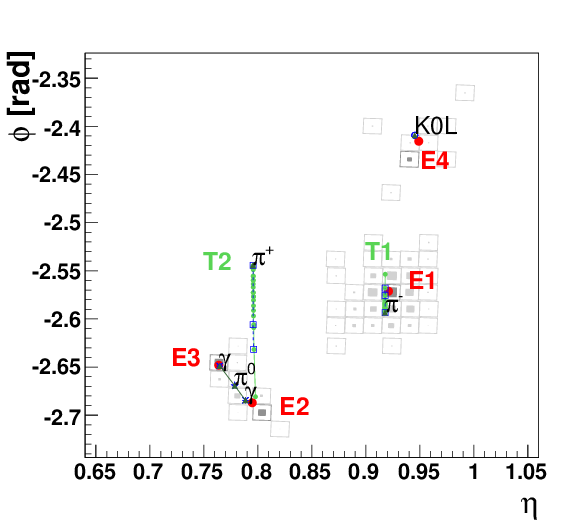
\includegraphics[width=.8\linewidth]{analysis/pics/PF_b.png}
		\caption{The $(\eta,\phi)$ view on ECAL.}
		\label{fig:PF_b}
	\end{subfigure}
	\begin{subfigure}{.4\textwidth}
		\centering
		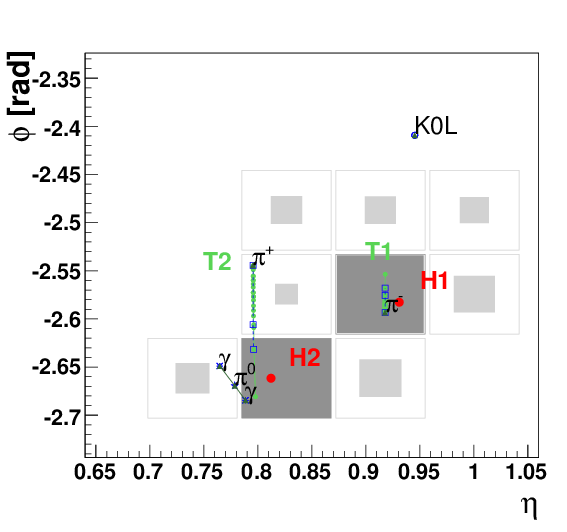
\includegraphics[width=.8\linewidth]{analysis/pics/PF_c.png}
		\caption{The $(\eta,\phi)$ view on HCAL.}
		\label{fig:PF_c}
	\end{subfigure}%
	\caption{An event display of a simple hadronic jet in the $(x, y)$ view (Figure \ref{fig:PF_a}) and in the $(\eta,\phi)$ view, where $\eta$ stands for pseudo-rapidity and $\phi$ for the azimuthal angle, on the ECAL surface (Figure \ref{fig:PF_b}) and the HCAL surface (Figure \ref{fig:PF_c}). (These two surfaces are represented as two circles centred around the interaction point in the first view.) The $K^{0}_{L}$, the $\pi^{-}$ and the two photons from the $\pi^{0}$ decay are detected as four well separated ECAL clusters (Figure \ref{fig:PF_b}). The $\pi^{+}$ leaves no energy in the ECAL. The two charged pions are reconstructed as charged-particle tracks, appearing as vertical solid lines in the $(\eta,\phi)$ views and circular arcs in the $(x, y)$ view. These tracks point towards two HCAL clusters (Figure \ref{fig:PF_c}). In all three views, the cluster positions are represented by dots, the simulated particles by dashed lines, and the position of their impact on the calorimeter surfaces by various open markers.}
	\label{fig:PF_event_display}
\end{figure}

Two algorithms are used to reconstruct \ptvecmiss, the imbalance in transverse momentum in the event, whose magnitude is referred to as \met. The standard algorithm computes the negative vectorial sum of all particle momenta reconstructed using the PF algorithm. In addition, a multivariate regression algorithm \cite{Khachatryan:2014gga} has been developed to reduce the effect of pileup on the resolution in \met. The algorithm utilizes the fact that pileup predominantly produces jets of low \pt, while leptons and high-\pt jets are produced almost exclusively in the hard-scatter. The transverse mass, \mt, of the system constituted by an electron or a muon and \met is used to either select or remove events that are due to W+jets and tt production. 

\clearpage

\section {The Tau Lepton reconstruction}

The $\tau$ lepton was discovered between 1974 and 1977 by the team under Martin Perl while studying the $e^{+}+e^{-}\longrightarrow e^{\pm}+\mu^{\mp}$. With a mean lifetime of $2.9\times10^{−13}$ s and a mass of 1776.82 \mev \cite{Agashe:2014kda} is the heaviest of the leptons, enough to decay into hadrons, and it does so in about two thirds of the cases, typically into either one or three charged pions or kaons and up to two neutral pions \ensuremath{\pi^{0}}, and one neutrino \ensuremath{\nu_{\tau}}. The \ensuremath{\pi^{0}} meson decays almost exclusively into \ensuremath{\gamma\gamma}. Among all the possible hadronic decays as shown on Table \ref{table:tau_hdecay} the ones called "one-prong", where only one charged hadron is produced, are the most frequent. The $\tau$ decays also leptonically, with a branching ratio of $17\%$ for each channel, via the following decay $\tau\longrightarrow\nu_{\tau}W^{*}\longrightarrow\nu_{\tau}l\nu_{l}$.

\begin{figure}[tbh!]
	\begin{center}	
		\begin{tabular}{ | c | c | c | c |}
			\hline
			Decay Mode & Resonance & Mass [\mev] & BF (\%) \\ \hline
			\hline
			$\tau^{-}\longrightarrow h^{-}\nu_{\tau}$& $\pi$ & 139.6 & 11.6 \\ \hline
			$\tau^{-}\longrightarrow h^{-}\pi^{0}\nu_{\tau}$& $\rho$ & 770 & 26.0 \\ \hline
			%				$\tau^{-}\longrightarrow h^{-}\pi^{0}\pi^{0}\nu_{\tau}$ & $a_{1}$ & 1200 & \\ 10.8 \hline
			$\tau^{-}\longrightarrow h^{-} h^{+} h^{-} \nu_{\tau}$& $a_{1}$& 1200 & 9.8 \\ \hline
			$\tau^{-}\longrightarrow h^{-} h^{+} h^{-} \pi^{0}\nu_{\tau}$& & & 4.8 \\ \hline
			other hadronic channels& & & 1.7 \\ \hline
			\hline
			total & & & 64.8 \\ \hline
			\hline
		\end{tabular}
		\caption{ Hadronic tau decay modes into either one or three charged hadrons h and potential $\pi_{0}$, and the corresponding branching fractions BF. Also shown are the intermediate resonances and their masses, which are used in some of the tau reconstruction algorithms.}
		\label{table:tau_hdecay}
	\end{center}
\end{figure}

\subsection{Algorithm for \hadtau reconstruction and identification}

The \hadtau decays are reconstructed and identified using the hadrons-plus-strips (HPS) algorithm \cite{Chatrchyan:2012zz} and is seeded by jets of \ensuremath{\pt > 14 \gev} and \ensuremath{|\eta| < 2.5}, reconstructed using the anti-\ensuremath{k_{T}} algorithm \cite{antikt} with a distance parameter of 0.5. The algorithm is designed to reconstruct individual decay modes of the \ensuremath{\tau} lepton, taking advantage of the excellent performance of the PF algorithm in reconstructing individual charged and neutral particles.
The reconstruction and identification of \hadtau decays in the HPS algorithm is performed in two steps:

\begin{itemize}
	\item \textbf{Reconstruction:} combinations of charged and neutral particles reconstructed by the PF algorithm that are compatible with specific \hadtau decays are constructed, and the four-momentum, expressed in terms of (\pt, \ensuremath{\eta}, \ensuremath{\phi} , and mass) of τh candidates, is computed.
	
	\item \textbf{Identification:} discriminators that separate \hadtau decays from quark and gluon jets, and from electrons and muons, are computed. This provides a reduction in the jet \ensuremath{\longrightarrow \hadtau}, \ensuremath{e \longrightarrow \hadtau}, and \ensuremath{\mu \longrightarrow \hadtau} misidentification rates.
\end{itemize}

\subsection{title}

Reconstruction of specific \hadtau decay modes requires reconstruction of neutral pions that are present in most of the hadronic \ensuremath{\tau} decays. The high probability for photons originating from \ensuremath{\pi^{0} \longrightarrow \gamma \gamma} decays to convert to \ensuremath{e^{+}e^{-}} pairs within the volume of the CMS tracking detector is taken into account by clustering the photon and electron constituents of the \ensuremath{\tau}-seeding jet into “strips” in the \ensuremath{\eta - \phi} plane. The clustering of electrons and photons of \ensuremath{\pt > 0.5} \gev into strips proceeds via an iterative procedure. The electron or photon of highest \pt not yet included into any strip is used to seed a new strip. The initial position of the strip in the \ensuremath{\eta - \phi} plane is set according to the \ensuremath{\eta} and \ensuremath{\phi} of the seed \ensuremath{e} or \ensuremath{\gamma}. The \ensuremath{e} or \ensuremath{\gamma} of next-highest \pt that is within an \ensuremath{\eta \times \phi} window centred on the strip location is merged into the strip. The strip position is then recomputed as an energy-weighted average of all electrons and photons contained in the strip:

\begin{equation}
\eta_{strip} = \dfrac{1}{\pt^{strip}} \sum \pt^{\gamma} \eta_{\gamma}
\end{equation}

\begin{equation}
\phi_{strip} = \dfrac{1}{\pt^{strip}} \sum \pt^{\gamma} \phi_{\gamma}
\end{equation}

with \ensuremath{\pt^{strip} = \sum \pt^{\gamma}}. The construction of the strip ends when no additional electrons or photons are found within an \ensuremath{\eta \times \phi} window of size \ensuremath{0.05 \times 0.20}. In which case the clustering proceeds by constructing a new strip, which is seeded by the \ensuremath{e} or \ensuremath{\gamma} with next highest \pt. The size of the window is enlarged in the \ensuremath{\phi} direction to account for the bending of \ensuremath{e^{+}} and \ensuremath{e^{-}} from photon conversions in the 3.8 T magnetic field. Strips with \pt sums of electrons and photons in the strip of \ensuremath{>2.5 \gev} are kept as \ensuremath{\pi^{0}} candidates.

Hadronic \ensuremath{\tau} candidates are formed by combining the strips with the charged-particle constituents of the jet. The charged particles are required to satisfy the condition \ensuremath{\pt > 0.5 \gev}. The distance of closest approach between their tracks and the hypothetical production vertex of the τh candidate, taken to be the vertex closest to the charged particle of highest \pt within the jet, is required to be less than 0.4 cm in the z direction and \ensuremath{< 0.03} cm in the transverse plane. The requirements for tracks to be compatible with the production vertex of the \ensuremath{\tau} removes spurious tracks and significantly reduces the effect of pileup, while being sufficiently loose so as not to lose efficiency because of the small distances that \ensuremath{\tau} leptons traverse between their production and decay.

\clearpage

\section {The Jet reconstruction}

